\begin{lstlisting}
from sie import *
\end{lstlisting}

\begin{lstlisting}
data=load_data('data/shoesize.xls')
\end{lstlisting}

\begin{lstlisting}
data.head()
\end{lstlisting}

\begin{verbatim}
   Index Gender  Size  Height
0      1      F   5.5      60
1      2      F   6.0      60
2      3      F   7.0      60
3      4      F   8.0      60
4      5      F   8.0      60
\end{verbatim}

\begin{lstlisting}
import random
\end{lstlisting}

\begin{lstlisting}
random.seed(102)
rows = random.sample(data.index, 10)
newdata=data.ix[rows]
data=newdata
data
\end{lstlisting}

\begin{verbatim}
     Index Gender  Size  Height
60      61      F   7.0      64
251    252      M   9.0      70
69      70      F   8.0      64
290    291      M  11.0      71
247    248      M  12.0      69
156    157      F   9.5      68
231    232      M  10.0      69
17      18      F   6.5      61
216    217      M  10.0      68
252    253      M   9.0      70
\end{verbatim}

\begin{lstlisting}
plot(data['Height'],data['Size'],'o')
gca().set_xlim([60,72])
gca().set_ylim([4,14])
xlabel('Height [inches]')
ylabel('Shoe Size')
\end{lstlisting}

\begin{verbatim}
<matplotlib.text.Text at 0x10adae0d0>
\end{verbatim}

\begin{center}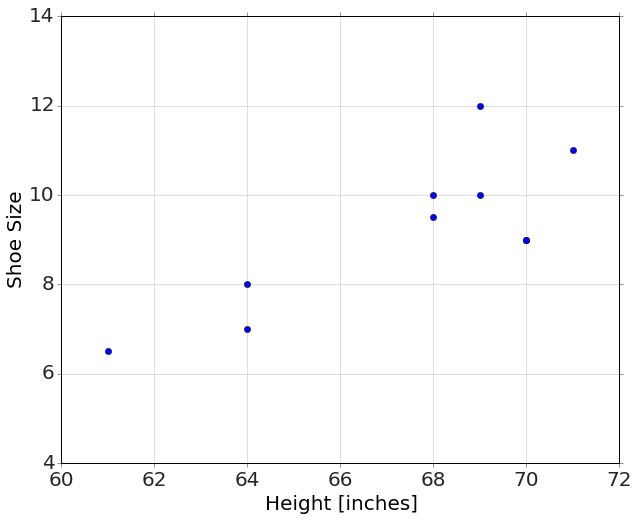
\includegraphics[width=4.5in]{Regression/Regression_fig0.png}\end{center}

\begin{lstlisting}
result=regression('Size ~ Height',data)
\end{lstlisting}

\begin{verbatim}
<matplotlib.figure.Figure at 0x10d200710>\end{verbatim}

\begin{center}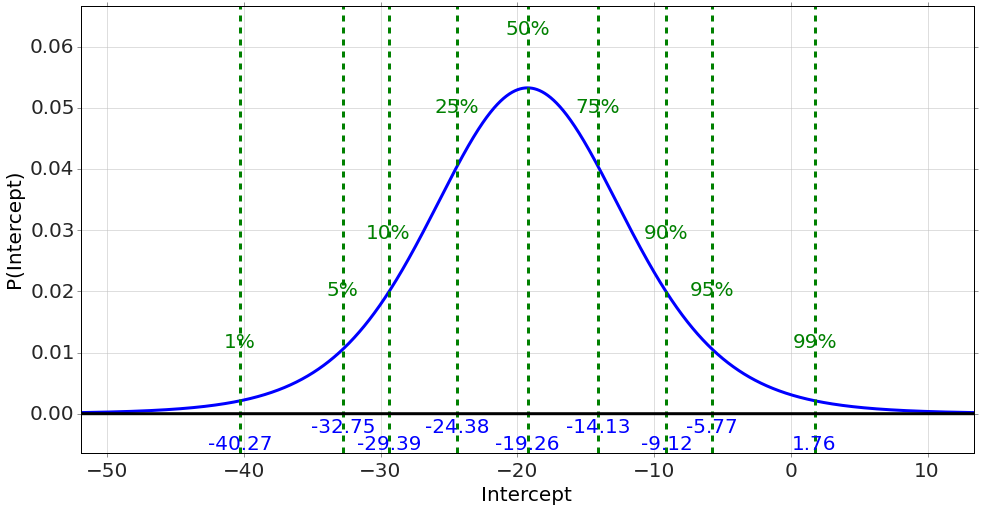
\includegraphics[width=4.5in]{Regression/Regression_fig1.png}\end{center}

\begin{verbatim}
<matplotlib.figure.Figure at 0x10d702610>\end{verbatim}

\begin{center}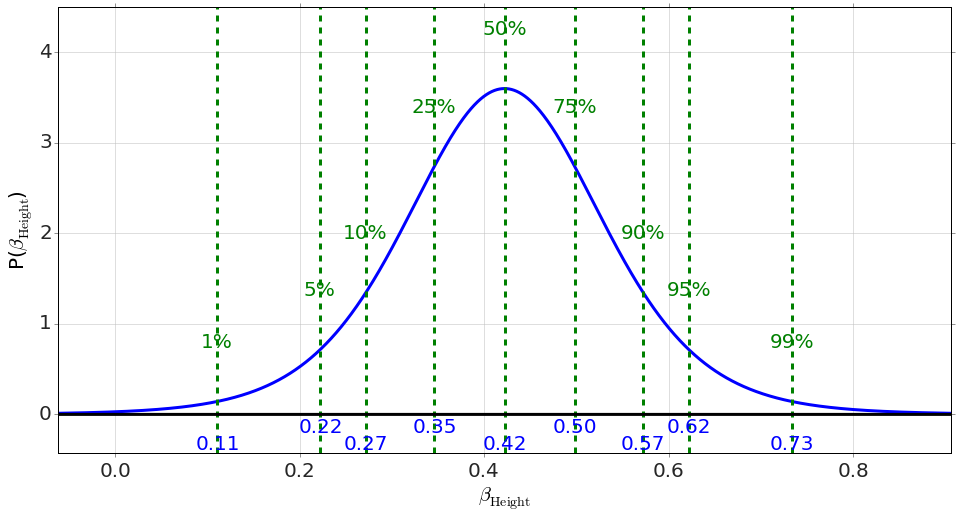
\includegraphics[width=4.5in]{Regression/Regression_fig2.png}\end{center}

\begin{lstlisting}
plot(data['Height'],data['Size'],'o')

h=linspace(60,72,10)
plot(h,result['_Predict'](Height=h),'-')

gca().set_xlim([60,72])
gca().set_ylim([4,14])
xlabel('Height [inches]')
ylabel('Shoe Size')

b=result.Intercept.mean()
m=result.Height.mean()

if b>0:
    text(62,12,'$y=%.3f x + %.3f$' % (m,b),fontsize=30)
else:
    text(62,12,'$y=%.3f x %.3f$' % (m,b),fontsize=30)
\end{lstlisting}

\begin{center}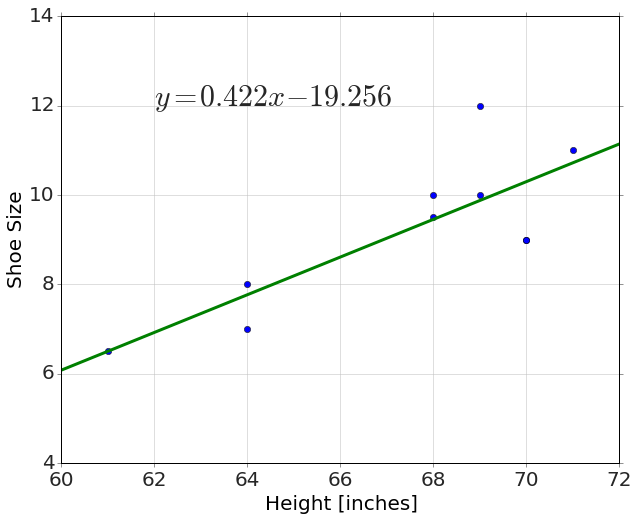
\includegraphics[width=4.5in]{Regression/Regression_fig3.png}\end{center}

\begin{lstlisting}
data=load_data('data/sat.csv')
\end{lstlisting}

\begin{lstlisting}
result=regression('total ~ expenditure',data)
\end{lstlisting}

\begin{verbatim}
<matplotlib.figure.Figure at 0x1109156d0>\end{verbatim}

\begin{center}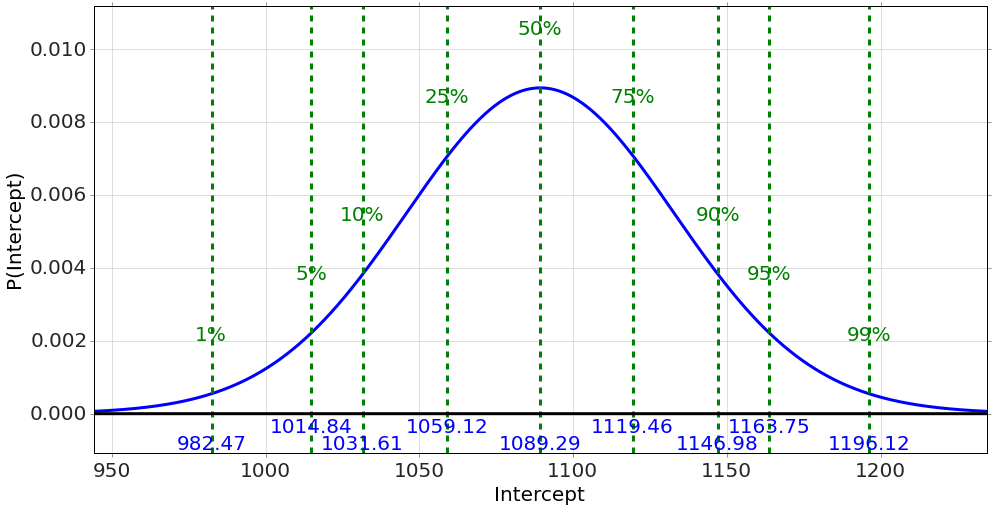
\includegraphics[width=4.5in]{Regression/Regression_fig4.png}\end{center}

\begin{verbatim}
<matplotlib.figure.Figure at 0x110953110>\end{verbatim}

\begin{center}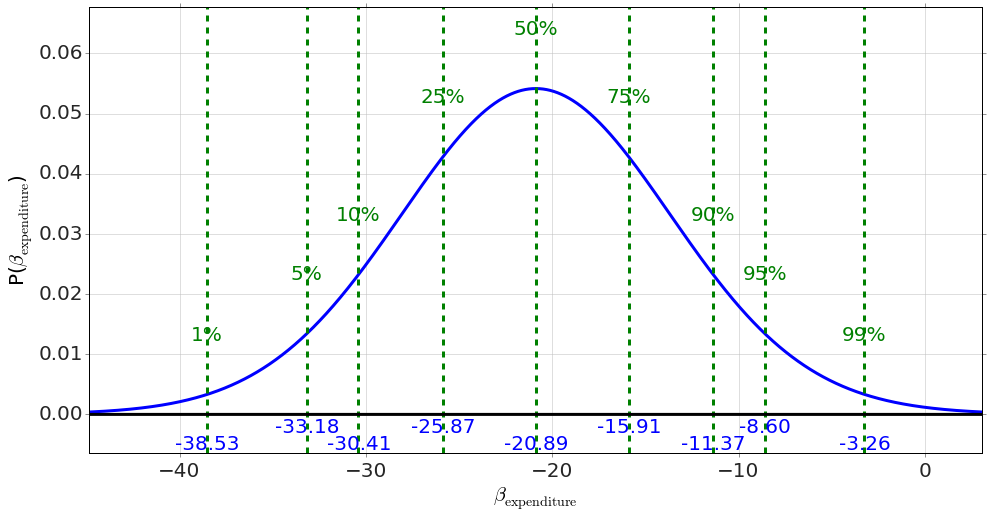
\includegraphics[width=4.5in]{Regression/Regression_fig5.png}\end{center}

\begin{lstlisting}
plot(data['expenditure'],data['total'],'o')
xlabel('Expenditure [per pupil, thousands]')
ylabel('SAT Total')
h=linspace(3,10,10)
plot(h,result['_Predict'](expenditure=h),'-')

b=result.Intercept.mean()
m=result.expenditure.mean()

if b>0:
    text(4.5,1125,'$y=%.3f x + %.3f$' % (m,b),fontsize=30)
else:
    text(4.5,1125,'$y=%.3f x %.3f$' % (m,b),fontsize=30)

\end{lstlisting}

\begin{center}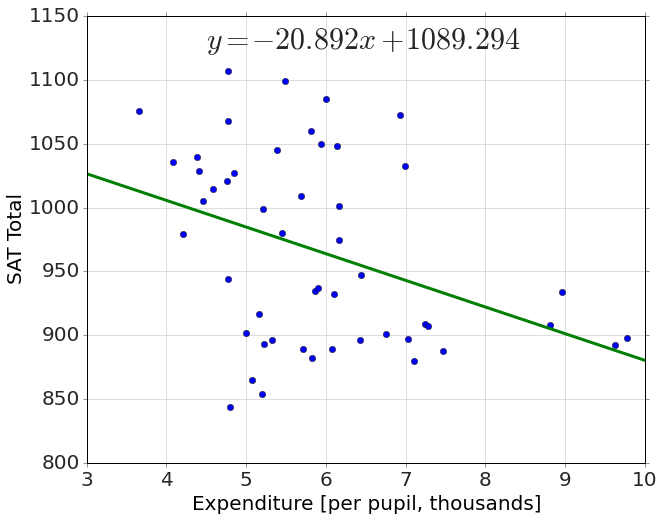
\includegraphics[width=4.5in]{Regression/Regression_fig6.png}\end{center}

\begin{lstlisting}
result=regression('percent_taking ~ expenditure',data)
\end{lstlisting}

\begin{verbatim}
<matplotlib.figure.Figure at 0x111cfff10>\end{verbatim}

\begin{center}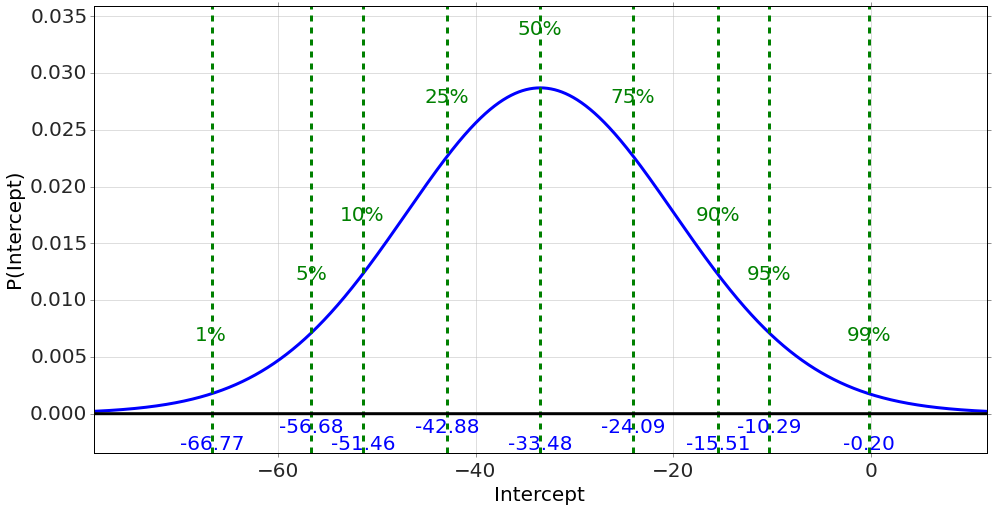
\includegraphics[width=4.5in]{Regression/Regression_fig7.png}\end{center}

\begin{verbatim}
<matplotlib.figure.Figure at 0x111867750>\end{verbatim}

\begin{center}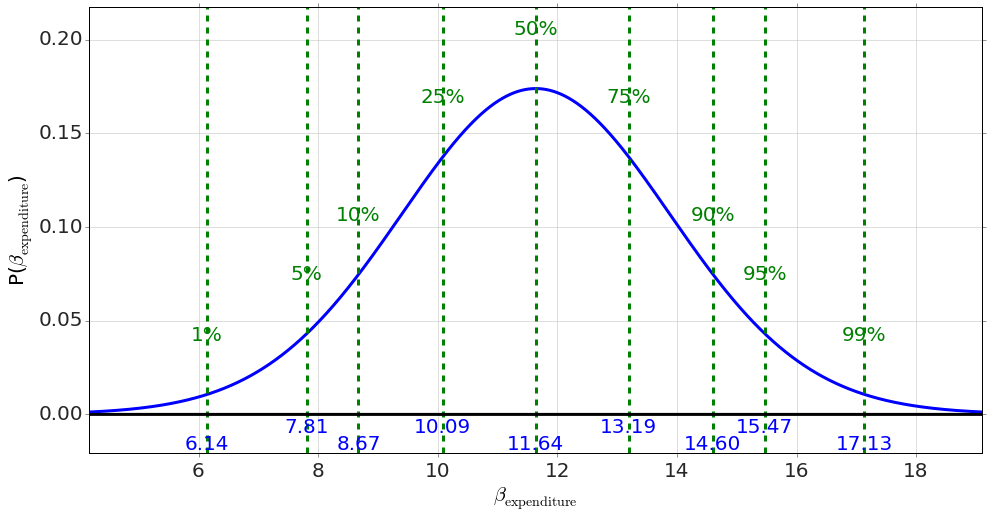
\includegraphics[width=4.5in]{Regression/Regression_fig8.png}\end{center}

\begin{lstlisting}
plot(data['expenditure'],data['percent_taking'],'o')
xlabel('Expenditure [per pupil, thousands]')
ylabel('SAT Total')
h=linspace(3,10,10)
plot(h,result['_Predict'](expenditure=h),'-')

b=result.Intercept.mean()
m=result.expenditure.mean()

if b>0:
    text(4.5,85,'$y=%.3f x + %.3f$' % (m,b),fontsize=30)
else:
    text(4.5,85,'$y=%.3f x %.3f$' % (m,b),fontsize=30)

\end{lstlisting}

\begin{center}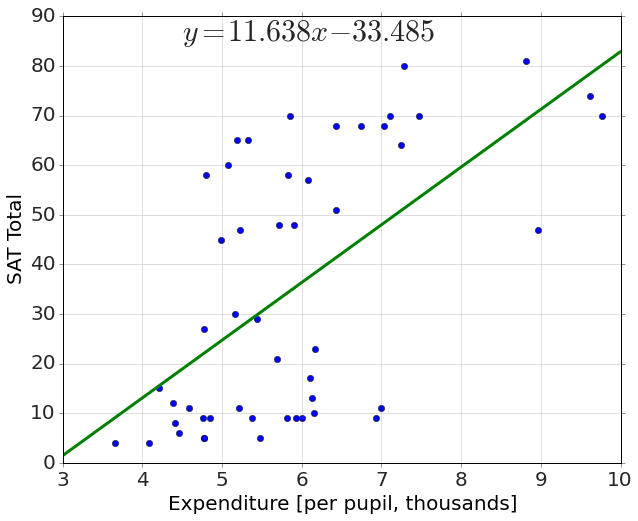
\includegraphics[width=4.5in]{Regression/Regression_fig9.png}\end{center}

\begin{lstlisting}
result=regression('total ~ expenditure + percent_taking',data)
\end{lstlisting}

\begin{verbatim}
<matplotlib.figure.Figure at 0x1107f5fd0>\end{verbatim}

\begin{center}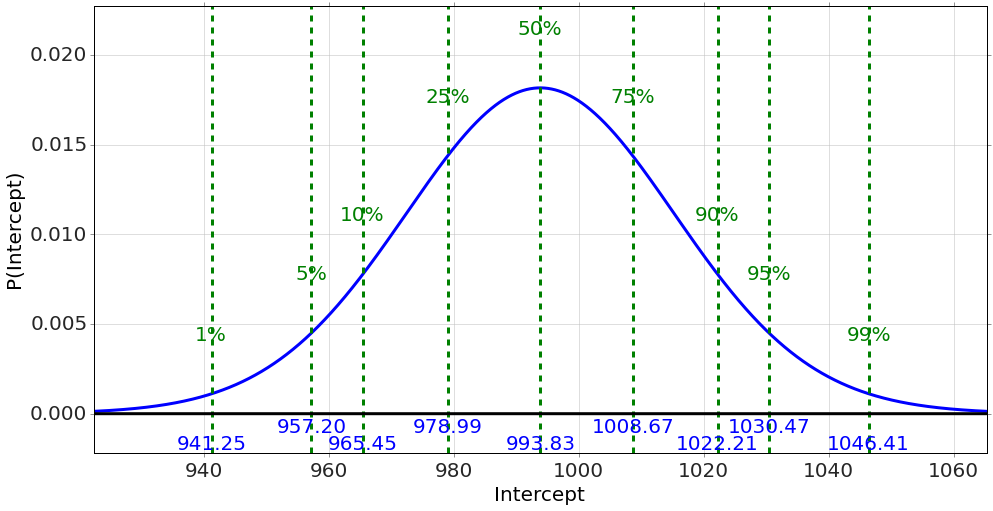
\includegraphics[width=4.5in]{Regression/Regression_fig10.png}\end{center}

\begin{verbatim}
<matplotlib.figure.Figure at 0x10d70a690>\end{verbatim}

\begin{center}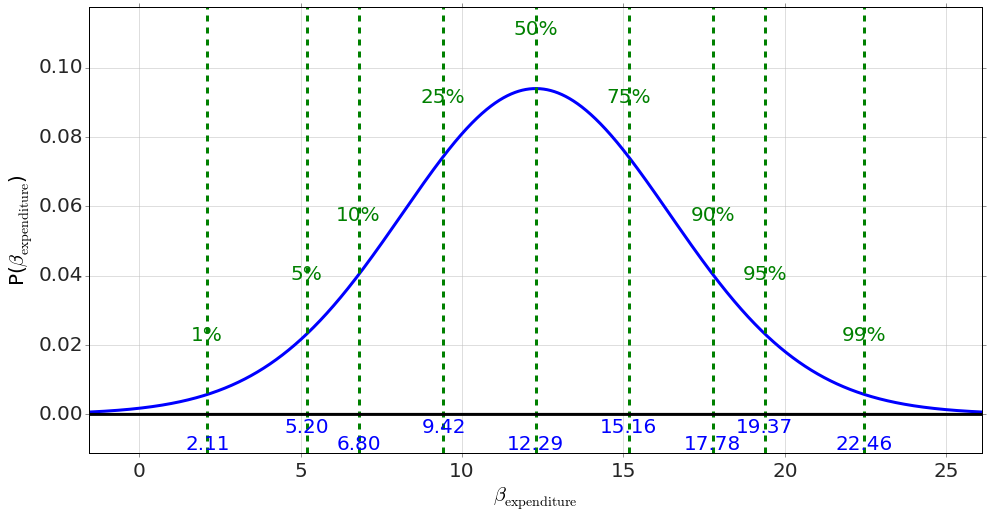
\includegraphics[width=4.5in]{Regression/Regression_fig11.png}\end{center}

\begin{verbatim}
<matplotlib.figure.Figure at 0x110fbcf90>\end{verbatim}

\begin{center}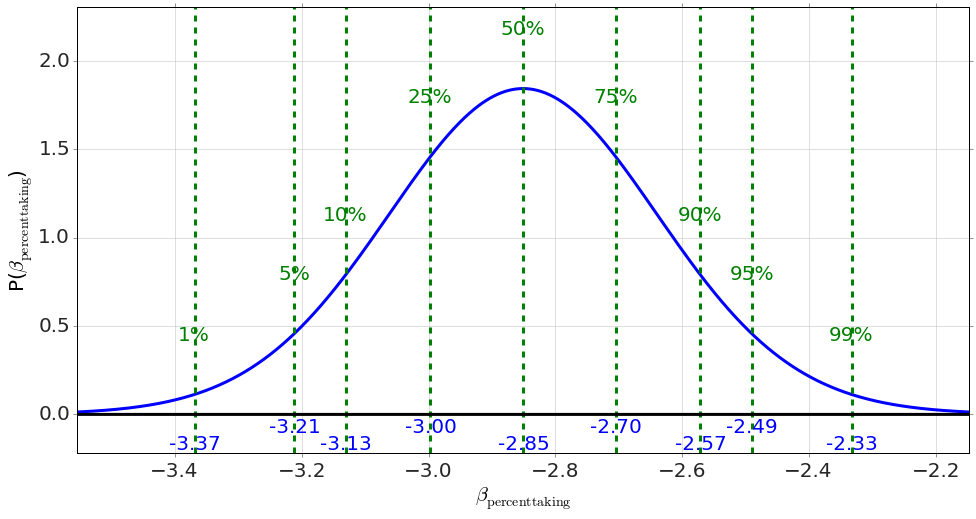
\includegraphics[width=4.5in]{Regression/Regression_fig12.png}\end{center}

\begin{lstlisting}

\end{lstlisting}

